\section{Real centre spectra with constructed context}
\label{sec:real}

\paragraph{What this experiment is.}
We test contextual competition using measured centre spectra and their
recorded labels, with a synthetic class-associated spatial intensity
pattern along training-estimated principal directions in the
neighbourhood. It asks whether the mechanism operates when the spectral
cue is a real, high-dimensional class contrast; natural neighbourhoods are
treated in Appendix~\ref{app:exp4}.

\paragraph{Data and readiness.}
Breast-tissue QCL micro-array cores, fold~0 of a five-fold patient-level
split; the binary task Cancer Epithelium versus Cancer-Associated Stroma
on $942$-channel pixel vectors; $24{,}000$ class-balanced training
centres; validation patients for evaluation, test patients reported
separately (Appendix~\ref{app:exp3}). A readiness scan
(Table~\ref{tab:exp3_scan}) shows that with per-feature standardization a
random encoder $W\in\R^{12\times942}$ already reads this contrast at
$0.955$ against a calibration discriminant of $0.969$; PCA
whitening estimated on the training patients reduces the random-encoder
probe to $0.54$ while the discriminant stays at $0.944$. We therefore run
two regimes on the same pixels and labels, \emph{high} and \emph{low
initial probe accessibility} (standardized and whitened inputs). Neither
is an instance of the theorem: a probe on the encoder output does not
measure the spectral contribution to a random head's margin.

\paragraph{Construction.}
Each patch is a real centre with eight real donor spectra drawn
independently of the centre label from the same split side; donor $d$
carries $\gamma_d(c\,s+\tau\eta_d)$ along the $d$th principal coordinate,
where $c$ is the centre's label, $s=\pm1$ or $c$ is replaced by an
independent label, and $\gamma_d$ is large relative to the donors'
natural variation ($3\sqrt{\lambda_d}$ standardized; $30$ in whitened
units, with a $\gamma=10$ variant declared before its runs). $\tau$ is
calibrated per regime so that a discriminant on the eight cue projections
matches the centre-only discriminant on training-side data ($0.969$ high,
$0.948$ low); through a random encoder the encoded patch, centre
included, reads at $0.94$--$0.99$. The model is the linear encoder over the nine
spectra and a ReLU head of width $M$ over the encoded patch, trained and
thresholded as in Section~\ref{sec:synthetic}; three registered seeds per
arm, with two added seeds agreeing (Appendix~\ref{app:exp3}).

\paragraph{Results: high accessibility.}
The probe is $0.91$--$0.94$ before training and changes little at
$L^\ast$ in any arm (gain $-0.015$ to $+0.035$), yet the
informative-context-trained heads are strongly context-reliant, with
reversal accuracy $0.08$--$0.10$ and context-random accuracy at chance
for every width and $\kappa$, all fitting within $70$--$230$ steps; the
uninformative-context comparator
reaches reversal $0.93$ and context-random $0.92$, the frozen encoder $0.09$
(Table~\ref{tab:exp3_ready}). A large deficit in this probe is not
necessary for failure.

\paragraph{Results: low accessibility.}
The probe starts at $0.56$--$0.60$. Among the $\gamma=30$
informative-context arms the mean gain at $L^\ast$ is at most $0.046$
(up to $0.10$ in one run), against $0.35$
for the uninformative-context comparator (probe $0.92$--$0.93$;
$15{,}000$--$17{,}000$ steps to $L^\ast$ against $59$--$226$); reversal
accuracy is $0.07$ against the comparator's $0.91$--$0.93$, the frozen
encoder giving $0.08$ (Table~\ref{tab:exp3_unready}). Slowing the head
gives only a small probe response (mean $+0.014$ from $\kappa=1$ to
$1/256$). The saved checkpoints show where the adaptation went: for every
seed and $\kappa$, $99.995$--$99.998\%$ of the squared net encoder update
lies in the span of the eight constructed-cue directions, against
$88$--$90\%$ under uninformative-context training
(Appendix~\ref{app:exp3}). That the cue's amplitude dominates the
encoder's own gradient is a supported hypothesis, not an identified
mechanism: the projection is not a pathwise gradient decomposition, and
the random head, unlike the theorem's zero-sum readout, lets contextual
learning proceed through the encoder even when the head barely moves.

\paragraph{Results: the lower-amplitude variant.}
At $\gamma=10$ the fit takes $530$--$1{,}800$ steps and the rate response
returns: the within-seed probe change from $\kappa=1$ to $1/256$ is
$+0.030$, $+0.049$, $+0.095$, against $+0.002$, $+0.023$, $+0.016$ at
$\gamma=30$ in the same seeds (paired difference positive in every seed),
while reversal stays at $0.06$--$0.08$ and the comparator again reaches
gain $0.35$, reversal $0.92$ (Table~\ref{tab:exp3_unready10}). The net update remains in the cue span
($99.96$--$99.98\%$): an amplitude-dependent accessibility response, not
the removal of contextual dominance.

\paragraph{Results: what retraining recovers.}
The recovery procedure of Section~\ref{sec:synthetic} separates the
regimes further (Table~\ref{tab:exp3_recovery}).
With high accessibility a fresh head retrained on decorrelated context
reaches reversal accuracy $0.90$--$0.96$ from every encoder, the random
initialization included, against $0.08$ for the original classifiers: the
spectral information was available and unused. At
$\gamma=30$ no encoder yields more than $0.45$--$0.56$; at $\gamma=10$ the
slow-head encoders yield $0.55$--$0.70$ against $0.48$--$0.60$ after the
fast head.

\paragraph{Reading.}
With measured spectra the outcome matches the synthetic experiment on
reliance: at every width and rate evaluated the original predictor uses
the constructed context when it is informative, with excess shifted risk
of $0.83$--$0.84$ over the uninformative-context comparator. On
adaptation it adds a scope condition: how much of the contrast the
encoder learns before the fit depends on the head's relative speed and on
the cue's amplitude, which are not interchangeable here. With the natural
$3\times3$ neighbourhoods of the same cores, which never straddle two
classes, the encoder learns the class signal equally with and without
informative context and the model uses the full spectrum, on tissue and
on a public scene (Appendices~\ref{app:exp4} and~\ref{app:pavia}).

\begin{figure}[t]
\centering
\IfFileExists{figures/fig4_exp3.pdf}{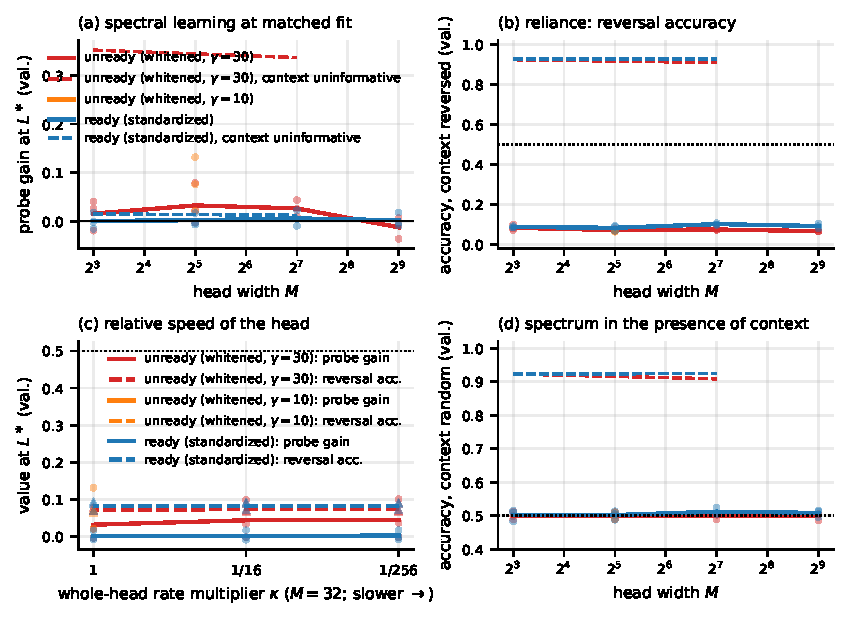
\includegraphics[width=\linewidth]{figures/fig4_exp3.pdf}}{\fbox{\rule{0pt}{2.0in}\rule{0.97\linewidth}{0pt}}}
\caption{Experiment 3 at $L^\ast=0.30$, validation patients, three seeds.
(a) Probe gain against width (high accessibility blue; low accessibility
$\gamma=30$ red, $\gamma=10$ orange; comparator dashed). (b) Reversal
accuracy. (c) Rate multiplier at $M=32$: probe gain (solid), reversal
(dashed). (d) Accuracy with uninformative context.}
\label{fig:exp3}
\end{figure}
